\chapter{Evaluierung}
Im letzten Teil dieser Arbeit wird mit den dynamische Experimenten die letzte Brücke zwischen Simulation und Realität geschlagen. Dazu wird ein Raum mit einem Scitos G5 vermessen und diese Daten in die Simulationsumgebung eingepflegt. Aus den gewonnenen Informationen wird eine Konfiguration für drei Beacons im Raum optimiert, geplant und installiert. Anschließend werden einzelne Koordinaten im Raum mit dem Roboter autonom angefahren und die jeweilige Signalstärke eines Beacons gemessen. Dabei werden die vorher getroffenen Annahmen aus den statischen Experimenten mit den neuen Erkenntnissen aus der dynamischen Disziplin miteinander verglichen. 
\section{Dynamisches Experiment}
In diesem letzten Experiment wird eine erstellte Beacon-Konfiguration auf ihre Ortungsgenauigkeit überprüft. Hierfür wird weniger auf die Vertrauensskala eingegangen, sondern die Signalstärken für einzelne Punkte im Raum aufgenommen, gespeichert und anschließend ausgewertet. In diesen Versuchen wird ausschließlich der Scitos G5 verwendet, weil er über eine eigene Lokalisierungsmöglichkeit verfügt und eine selbstständige Pfadplanung durchführen kann. Somit stellt seine Positionsschätzung die Referenz zu der beaconbasierten dar. Die Koordinaten die er ansteuert, kommen dabei aus der Simulationsumgebung als Mittelpunkte der Raumelemente. In diesem Test wird das ROS-Framework für die Kommunikation aller Geräte genutzt und wie in der Konzeptplanung in Abschnitt \ref{fig:SoftArch} gefordert wurde hier umgesetzt.
\subsection{Durchführung}
Im Experiment wird ein Adapter, der Daten zwischen dem Miracenter und ROS übertragen kann, benötigt. Dazu wird eine vorgefertige Software namens "`Scitos Metralabs"' \cite{SciMetra} verwendet, die die zweidimensionalen Raumkoordinaten vom Scitos an den ROS-Sever sendet und von diesem auch Zielkoordinaten entgegennehmen kann. Zur weiteren Vorbereitung zählt der Aufbau eines Raumes. Aufgrund des Mangels an großen Räumen ohne Interieur in der Universität, wurde kurzerhand ein Hörsaal umfunktioniert und die "`Wände"' mit auf der Seite liegenden Tischen aufgebaut. Der dadurch entstandene Grundriss besitzt die Abmessungen von 11,9 $\times$ 7 Meter. Dieser wird mithilfe des Roboters manuell kartografiert und als Bilddatei gespeichert (siehe Abbildung \ref{fig:Grundrisszeichnung}). Die Höhe der Tischkanten reicht dabei aus, um als Hindernis bzw. Wand vom dem Scitos wahrgenommen zu werden. Im Vergleich zur Zeichnung des Grundrisses ist in Abbildung \ref{fig:BildvomRaum} der Aufbau als Fotografie festgehalten. Dabei ist auch in der Mitte des Fotos der Scitos G5 zu erkennen.
\begin{figure}[H] 
$\begin{minipage}[b]{7.5cm}
\centering

\includegraphics[scale=0.8]{Bilder/Masterraum.png}
\caption{Grundriss des Testraumes}
\label{fig:Grundrisszeichnung}
\end{minipage}
\hfill
\begin{minipage}[b]{7.5cm}
\centering
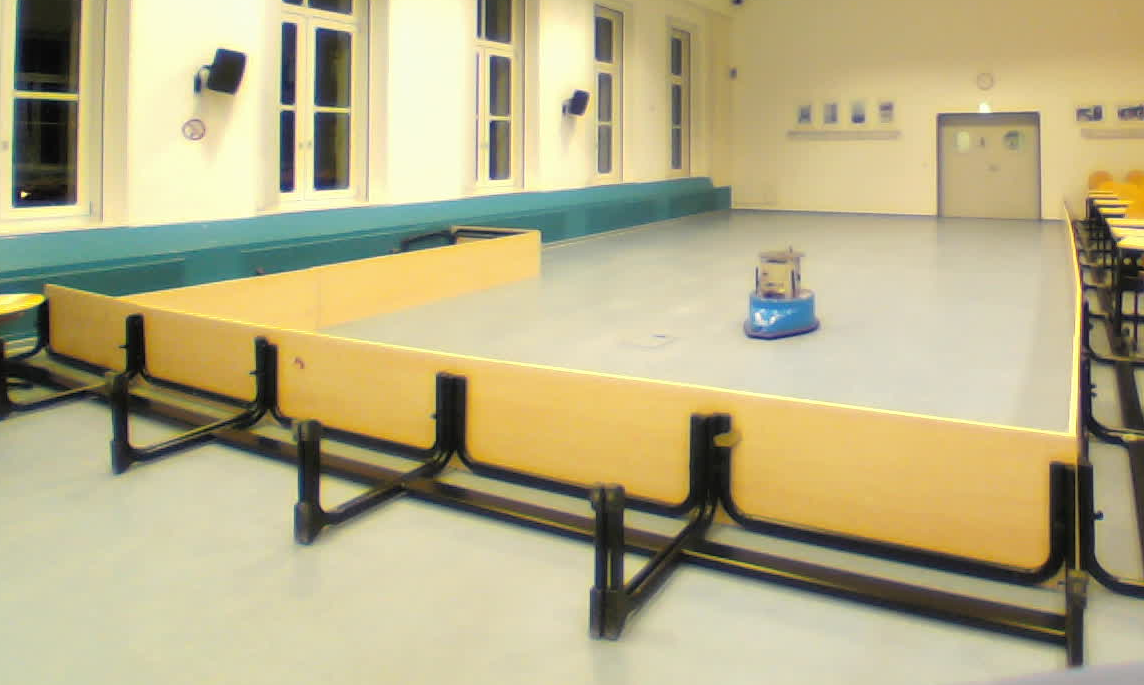
\includegraphics[scale=0.18]{Bilder/BildvomRaum}
\caption{Foto des Testraumes}
\label{fig:BildvomRaum}
\end{minipage}$
\end{figure}
Es wird dabei sehr gut ersichtlich, dass die künstlichen Wände nicht gerade verlaufen. Zudem ist der Grundriss mit kleinen Fragmenten und Fehlern behaftet, weswegen die Zeichnung in dieser Form nicht von der Simulationsumgebung verarbeitet werden kann. Deswegen muss jede Karte nachträglich geändert werden, indem die Wände begradigt und die kleinen Fragmente entfernt werden. Hierfür wurde ein normales Bildbearbeitungsprogramm verwendet und das Ergebnis aus der Änderung ist in Abbildung \ref{fig:Masterraum2} zu sehen.  
\begin{figure}[H] 
\centering

\includegraphics[scale=0.8]{Bilder/Masterraum2}
\caption{Bearbeiteter Grundriss}
\label{fig:Masterraum2}
\end{figure}
\subsection{Einsatz des Lighthouse Keepers}
Aus dem erstellten Grundriss werden optimale Beacon-Konfigurationen mithilfe des Lighthouse Keepers erstellt. Die Wahl der Parameter orientiert sich hierbei an den Einstellungen des Testbeispiels aus Abschnitt \ref{sec:Simulationsbeispiel}. Lediglich die Toleranz wird auf $1,5$ Meter erhöht, damit der Roboter sicher wenden und die vorgegebenen Positionen ansteuern kann. Das Ziel der Planung in diesem Experiment ist es, alle verfügbaren Beacons anzubringen, damit in einem Durchlauf so viele Daten wie möglich gesammelt werden. Das Ergebnis der Simulation und Optimierung für drei Beacons findet sich in der unten stehenden Abbildung \ref{fig:BeacKon}.
\begin{figure}[H] 
\centering
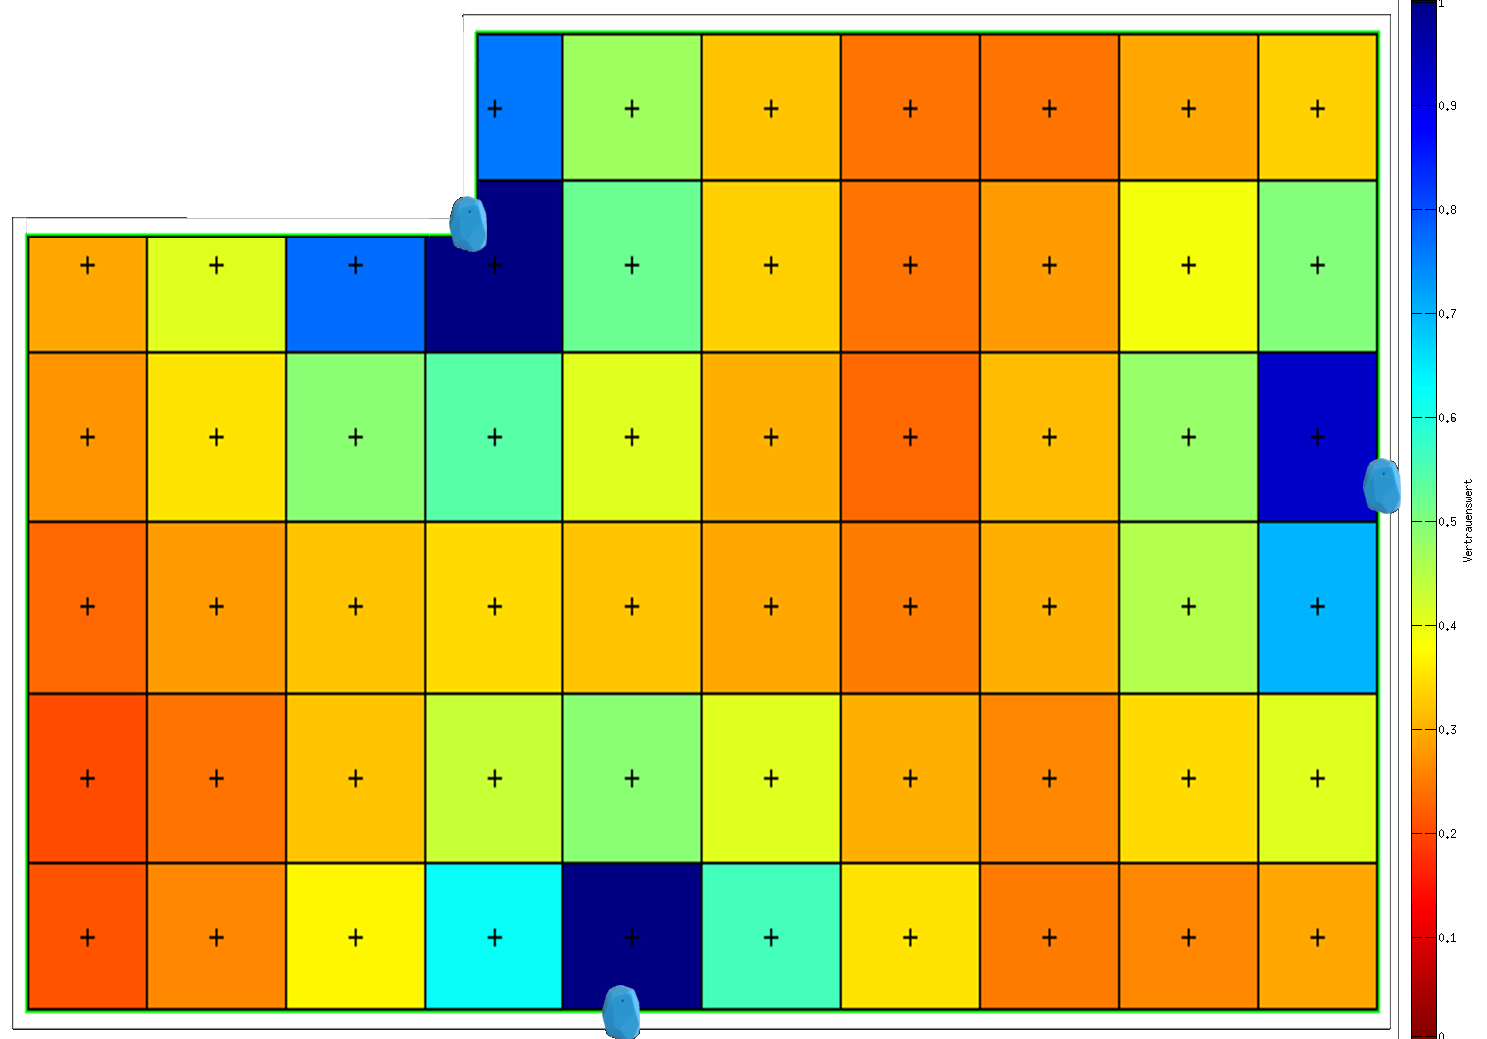
\includegraphics[scale=0.22]{Bilder/SimMasterraum}
\caption{Beacon-Konfiguration der dynamischen Experimente}
\label{fig:BeacKon}
\end{figure}
\subsection{Pfadplanung und Navigation}
Die Positionen der Raumelemente und Befestigungspunkten werden in der Simulation als Textdokument gespeichert, sodass der Mira-ROS-Adapter ständig auf diese während des Experimentes zugreifen kann. Die Mittelpunkte der Raumelemente dienen als Kette von Punkten, die der Adapter einzeln an die Navigation des Scitos Roboters sendet. Speziell dafür wird eine Abfrage in den Adapter implementiert, die den nächsten Punkt auf der Trajektorie mit der aktuellen Position des Roboters vergleicht. Befindet sich der Roboter an den Koordinaten des angesteuerten Raumelementes, wird eine Wartezeit von zehn Sekunden vorgegeben. Nach Ablauf der Zeit überträgt der Adapter den nachfolgenden Punkt in der Textdatei und der Roboter fährt die nächsten Koordinaten an usw.. \\ \\
Die komplette Durchführung wurde in einem Zeitraffer-Video festgehalten und findet sich auf der beigelegten CD-ROM oder im Internet unter: \url{https://www.youtube.com/watch?v=_IeiKjpdh18}.  
\section{Auswertung}
Wie zum Anfang erwähnt wurde, setzt das Lighthouse Keeper-Prinzip auf den Scitos G5 und seiner internen Positionsbestimmung. Bei der Betrachtung der Positionsdaten vom Roboter fiel ein starker Drift der Daten bei fortschreitender Dauer des Experimentes auf. In Abbildung \ref{fig:Drift} ist dies einmal dargestellt. Die blaue Linie stellt die Bewegung des Roboters dar und der Startpunkt liegt mittig links. Im Video wird sehr gut ersichtlich, dass der Roboter alle Punkte entlang der Trajektorie zielsicher anfährt. In dem Experiment fuhr er dabei von oben links nach unten rechts. Die Daten, die der Roboter hingegen über seine Middleware an ROS weitergibt, spiegeln in keinster Weise das Verhalten aus dem Video wieder. 
\begin{figure}[H] 
\centering
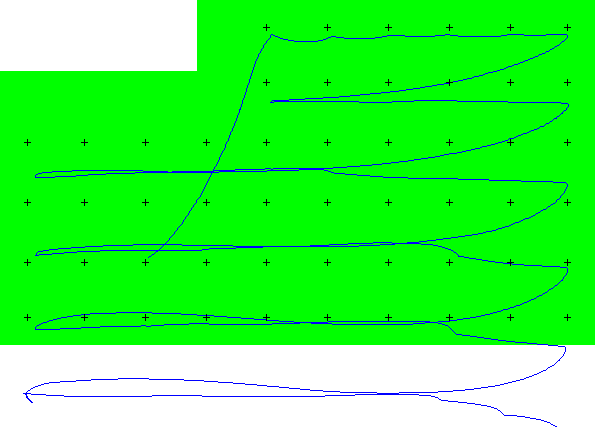
\includegraphics[scale=0.38]{Bilder/Drift}
\caption{Drift des Scitos G5}
\label{fig:Drift}
\end{figure}
In der Abbildung ist zu erkennen, wie er Roboter (rein virtuell) den Raum sogar verlässt. Eine wahrscheinliche Begründung für die schlechte Ortung könnte das Interesse der Entwickler vom Miracenter sein, ihre Software und Ideen schützen zu wollen, indem sie die internen Vorgänge in der Navigations-Toolbox nicht preisgeben. Die gesendete Positionsdaten stammen mit hoher Wahrscheinlichkeit nur von den Odometrie-Sensoren. Die Verarbeitung aller Bewegungs- und Distanzsensoren geschieht (wahrscheinlich) nur für die eigene Navigation. Trotzdem müssen diese Daten für den Lighthouse Keeper aufbereitet werden, damit eine gute Referenzortung gegeben ist. Deswegen wird für die Beseitigung des Drifts ein weiteres Verfahren benötigt, das gerade diesen schätzt. Das Problem wird hier wieder als Optimierungsaufgabe formuliert. Die Kostenfunktion leitet sich dabei aus der Differenz eines Stopppunktes $P$ des Roboters zu den Koordinaten des angestrebten Zielpunktes $M$ (der Mittelpunkt von einem Raumelement) ab. Wiederum wird diese Funktion aus den bekannten Vorteilen quadriert. Die zu optimierenden Parameter $a$ und $b$ werden zur Berechnung des Drifts in eine Wachstumsfunktion eingesetzt. Die Annahme dahinter ist das lineare Wachstum des Drifts mit zurückgelegtem Weg $d$ in den x- und y-Richtung. 
\begin{align*}
d_i &=d_{i-1}+\sqrt{\left (P_i-P_{i-1}  \right )^2} \qquad \text{mit} \qquad d_0,\, P_0=0\\
P_{neu,i} &=\begin{pmatrix}
a\cdot d_i + P_{i,x}\\ 
b\cdot d_i + P_{i,y}
\end{pmatrix}\\
\underset{a,b}{\min} \; J &= \sum_{i=1}^{n}\left ( M_i - P_{neu,i} \right )^2
\end{align*}
Als Optimierungsverfahren wird wieder der bewährte PSO genutzt. In den Abbildungen \ref{fig:OptiDrift1} bis \ref{fig:NoDrift} ist das Ergebnis der Bemühungen dargestellt. Es ist sehr gut ersichtlich, dass der lineare Ansatz funktioniert und im Vergleich zum Video das Verhalten sehr gut abgebildet ist. Weil der Zugriff auf die internen Positionsdaten vom Scitos verwährt bleibt, ist keine 100 prozentige Garantie gegeben, dass die Daten übereinstimmen. Für die Referenzgebung im Falle der Indoor-Lokalisierung reicht die gewonnene Qualität der Positionsbestimmung weitesgehend aus. 
\begin{figure}[H] 
$\begin{minipage}[t]{7.5cm}
\centering
\begin{tikzpicture}
\begin{axis}[width=0.45\paperwidth, height=0.25\paperheight, y dir=reverse, hide axis, legend pos=north west]
\addplot+[color=blue, only marks,mark=x,semithick] table [col sep=comma] {TikzDaten/DriftFinger.dat}; 
\addplot+[color=black, only marks, mark=o, semithick] table [col sep=comma] {TikzDaten/NoDrift1.dat};
\legend{Zielpunkte,Haltepunkte};
\end{axis}
\end{tikzpicture}
\caption{Haltepunkte mit Drift}
\label{fig:OptiDrift1}
\end{minipage}
\hfill
\begin{minipage}[t]{7.5cm}
\centering
\begin{tikzpicture}
\begin{axis}[width=0.45\paperwidth, height=0.25\paperheight, y dir=reverse, hide axis]
\addplot+[color=white, only marks, mark=o, semithick] table [col sep=comma] {TikzDaten/NoDrift1.dat};
\addplot+[color=blue, only marks,mark=x,semithick] table [col sep=comma] {TikzDaten/DriftFinger.dat}; 
\addplot+[color=black, only marks, mark=o, semithick] table [col sep=comma] {TikzDaten/NoDrift2.dat};
\end{axis}
\end{tikzpicture}
\caption{Haltepunkte ohne Drift}
\label{fig:OptiDrift2}
\end{minipage}$
\end{figure}
\begin{figure}[H] 
\centering
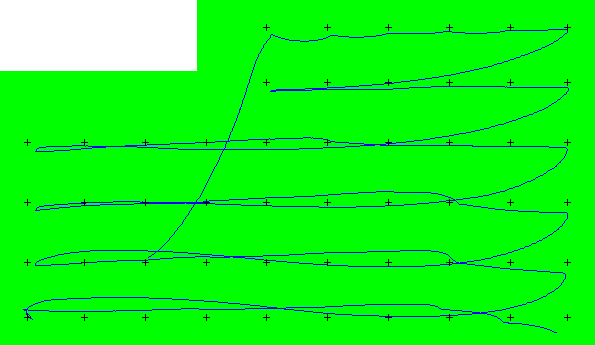
\includegraphics[scale=0.38]{Bilder/NoDrift}
\caption{Beseitigung vom Drift}
\label{fig:NoDrift}
\end{figure}
Nachdem die driftlosen Positionsdaten zur Verfügung stehen, wird im Folgenden mit der Auswertung der Beacon-Signalen begonnen. Als erstes wird dazu in den Abbildungen \ref{fig:DynAus1}, \ref{fig:DynAus2} und \ref{fig:DynAus3} die Distanz von Roboter bzw. Smartphone zu einem Beacon über die Zeit aufgetragen und dazu die empfangene Signalstärke gegenüber gestellt. Ferner ist neben der gemessenen Signalstärke auch die geschätzte aus dem WIINER II-Modell in das Diagramm eingetragen. Die Messungen aus den dynamischen Experimenten verhalten sich dabei ähnlich wie die der statischen Versuchen. Signifikant ist dafür die Übereinstimmung von prädiktioniertem Ausbreitungsverlust zu dem realen. Lediglich nach zehn Minuten driften beide Verläufe voneinander weg. Dies wird daran liegen, dass der Drift aus der Odometrie nicht gänzlich verschwunden ist und dadurch der Referenzabstand ungenauer wird.  
\begin{figure}[H] 
\centering
\begin{tikzpicture}
\begin{groupplot}[group style={group name=my plots, group size=1 by 2,ylabels at=edge left, vertical sep= 1.5cm}, width=0.7\paperwidth, height=0.15\paperheight, tickpos=left, ytick align=outside, xtick align=outside, enlarge x limits=false]
\nextgroupplot[title={Distanz Beacon zu Roboter},ylabel={Distanz in Meter},xticklabels={,,}]
\addplot[color=black] table [col sep=comma] {TikzDaten/DisDynAus1.dat};
\nextgroupplot[title={Signalstärke},ylabel={RSSI in dBm},xlabel={Zeit in Sekunden}, y dir=reverse, legend style={at={(0.9,-0.1)},anchor=south}]
\addplot[color=blue] table [col sep=comma] {TikzDaten/RSSIDynAus1.dat};
\addplot[color=red] table [col sep=comma] {TikzDaten/RSSIoptiDynAus1.dat};
\legend{gemessene Werte,Modellwerte};
\end{groupplot}
\end{tikzpicture}
\caption{Zeitlicher Verlauf der Signalstärke und des Abstandes für Beacon 1}
\label{fig:DynAus1}
\end{figure}
\vfill
\begin{figure}[H] 
\centering
\begin{tikzpicture}
\begin{groupplot}[group style={group name=my plots, group size=1 by 2,ylabels at=edge left, vertical sep= 1.5cm}, width=0.7\paperwidth, height=0.15\paperheight, tickpos=left, ytick align=outside, xtick align=outside, enlarge x limits=false]
\nextgroupplot[title={Distanz Beacon zu Roboter},ylabel={Distanz in Meter},xticklabels={,,}]
\addplot[color=black] table [col sep=comma] {TikzDaten/DisDynAus2.dat};
\nextgroupplot[title={Signalstärke},ylabel={RSSI in dBm},xlabel={Zeit in Sekunden}, y dir=reverse, legend style={at={(0.9,-0.15)},anchor=south}]
\addplot[color=blue] table [col sep=comma] {TikzDaten/RSSIDynAus2.dat};
\addplot[color=red] table [col sep=comma] {TikzDaten/RSSIoptiDynAus2.dat};
\legend{gemessene Werte,Modellwerte};
\end{groupplot}
\end{tikzpicture}
\caption{Zeitlicher Verlauf der Signalstärke und des Abstandes für Beacon 2}
\label{fig:DynAus2}
\end{figure}
\begin{figure}[H] 
\centering
\begin{tikzpicture}
\begin{groupplot}[group style={group name=my plots, group size=1 by 2,ylabels at=edge left, vertical sep= 1.5cm}, width=0.7\paperwidth, height=0.15\paperheight, tickpos=left, ytick align=outside, xtick align=outside, enlarge x limits=false]
\nextgroupplot[title={Distanz Beacon zu Roboter},ylabel={Distanz in Meter},xticklabels={,,}]
\addplot[color=black] table [col sep=comma] {TikzDaten/DisDynAus3.dat};
\nextgroupplot[title={Signalstärke},ylabel={RSSI in dBm},xlabel={Zeit in Sekunden}, y dir=reverse, legend style={at={(0.9,-0.1)},anchor=south}]
\addplot[color=blue] table [col sep=comma] {TikzDaten/RSSIDynAus3.dat};
\addplot[color=red] table [col sep=comma] {TikzDaten/RSSIoptiDynAus3.dat};
\legend{gemessene Werte,Modellwerte};
\end{groupplot}
\end{tikzpicture}
\caption{Zeitlicher Verlauf der Signalstärke und des Abstandes für Beacon 3}
\label{fig:DynAus3}
\end{figure}
\section{Diskussion}
Die Ergebnisse haben gezeigt, dass das Modell für die Ausbreitungsverluste sehr gut ausgelegt ist. Die Modellwerte bilden eine Grenze für die Maximalwerte der empfangbaren Signalleistung für alle Distanzen. Somit muss der Nutzer des Lokalisierungssystems lediglich auf das stärkste Signal warten. Die Simulationsumgebung positioniert dabei die Beacons so, dass die Wartezeiten auf ein gültiges Signal so kurz wie möglich sind. Jedoch konnte im Verlauf des dynamischen Experiments nicht auf die Vertrauensskala eingegangen werden. Hierbei wird der größte konzeptionelle Unterschied zwischen beiden Versuchsarten deutlich. Während mit den statischen Untersuchungen das Langzeitverhalten von Beacons untersucht wird, kommt es bei Evaluierung der Konfiguration auf die Geschwindigkeit an. Schließlich sollen ganze Gebäude auf die vollständige Abdeckung mit Beacons überprüft werden und der Testraum mit seinen 80 m$^2$ hat über 20 Minuten in Anspruch genommen. Die Zeit die ein Roboter für die Evaluierung benötigt, könnte sicherlich noch verkürzt werden, indem die Raumelemente größer ausgelegt werden und die Wartezeit an einem Haltepunkt minimiert wird. Es hat sich bei der Auswertung der Daten ergeben, dass keine Unterschiede zwischen dem ruhenden Roboter und dem fahrenden Roboter bezüglich des Signalempfanges bestehen. Die Streuung der RSSI-Werte hat in der Fahrt weder zugenommen, noch hat sich die Empfangsqualität verschlechtert. 